\documentclass[x11names,12pt,openright,twoside]{report}
\usepackage[a4paper,top=25mm,bottom=25mm,right=25mm,left=25mm,bindingoffset=6mm]{geometry}
\usepackage[utf8]{inputenc}
\usepackage[british]{babel}
\usepackage{amsmath}
\usepackage{graphicx}
\usepackage[dvipsnames]{xcolor}
\usepackage{pict2e}
\usepackage{tabu}
\usepackage{booktabs}
%\usepackage{bookmark,hyperref}
\usepackage[hypertexnames=true]{hyperref}
%\usepackage{hyperref}
\usepackage{gensymb}
\usepackage{wrapfig}
\usepackage{multirow}
\usepackage[nottoc]{tocbibind}


\usepackage{colortbl}
%\usepackage[table]{xcolor}
%\usepackage{tabularray}
\usepackage{watermark}
\usepackage{wallpaper}
\usepackage{eurosym}
\usepackage[toc,title,page]{appendix}
\usepackage{courier}
\usepackage{listings} 
\usepackage{enumitem}
\usepackage{url}
\usepackage{soul}
\usepackage{comment}
\usepackage{parskip}
\usepackage{etoolbox}
\usepackage{textcomp}
\usepackage{float}
\usepackage{xcolor}
%\usepackage{lststyle-VS2017.sty}

%\usepackage{minted} 


%\usepackage{fontspec}
\graphicspath{{figuren/}}


\definecolor{mygray}{gray}{0.85}

\newcommand{\ctext}[3][RGB]{%
	\begingroup
	\definecolor{hlcolor}{#1}{#2}\sethlcolor{hlcolor}%
	\hl{#3}%
	\endgroup
}


\newcommand{\specialcell}[2][c]{%
	\begin{tabular}[#1]{@{}c@{}}#2\end{tabular}}

\newcommand*{\img}[1]{%
	\raisebox{-.3\baselineskip}{%
		\includegraphics[
		height=\baselineskip,
		width=\baselineskip,
		keepaspectratio,
		]{#1}%
	}%
}
\newcommand*{\imgl}[1]{%
	\raisebox{-.3\baselineskip}{%
		\includegraphics[
		height=\baselineskip,
		%		width=\baselineskip,
		keepaspectratio,
		]{#1}%
	}%
}

%Formatering av rubriker
%%%%%%%%%%%%%%%%%%%%%%%%%%%%%%%%%%%%%%%%%%%%%%%%%%%%%%%%%%%%%%%%%%%%%%%%%%%%%%%%%%%%%%%
\usepackage{titlesec, blindtext, color}
\titleformat{\chapter}[hang]{\Huge\bfseries}{\thechapter}{20pt}{}{}
\titlespacing*{\chapter}{0pt}{*0}{*3}
\titlespacing*{\section}{0pt}{*4}{*1}
\titlespacing*{\subsection}{0pt}{*3}{*0}
\titlespacing*{\subsubsection}{0pt}{*4}{*1}

\setcounter{secnumdepth}{2}
\setcounter{tocdepth}{2}
%%%%%%%%%%%%%%%%%%%%%%%%%%%%%%%%%%%%%%%%%%%%%%%%%%%%%%%%%%%%%%%%%%%%%%%%%%%%%%%%%%%%%%%

\usepackage{tocloft} %Control the ToC formatting

\setlength{\parindent}{0pt}
\setlength{\parskip}{1em}

\lstset{ 
	basicstyle=\ttfamily\footnotesize,
	language=C++,
	        keywordstyle=\color{blue},
	stringstyle=\color{red},
	commentstyle=\color{green},
	morecomment=[l][\color{magenta}]{\#},
    captionpos=b,
    tabsize=3
}


%Formatting of page numbering (Comment to have the number centered)
%%%%%%%%%%%%%%%%%%%%%%%%%%%%%%%%%%%%%%%%%%%%%%%%%%%%%%%%%%%%%%%%%%%%%%%%%%%%%%%%%%%%%%%
\usepackage{fancyhdr}
\pagestyle{fancyplain}%
\fancyhf{} % clear all header and footer fields
\fancyfoot[RO,LE]{\thepage}
\renewcommand{\headrulewidth}{0pt}
%%%%%%%%%%%%%%%%%%%%%%%%%%%%%%%%%%%%%%%%%%%%%%%%%%%%%%%%%%%%%%%%%%%%%%%%%%%%%%%%%%%%%%%


\usepackage[font=footnotesize,format=plain,labelfont=bf,textfont=sl]{caption}
\usepackage[labelformat=simple,font=footnotesize,format=plain,labelfont=bf,textfont=sl]{subcaption}

\hypersetup{
	colorlinks=true,
	linkcolor=blue,
	filecolor=magenta,      
	urlcolor=cyan,
	pdfnewwindow=true, 
}
%opening
%  \date{\today}
\date{}
\title{
	
	{\vspace{-4cm}}
	
	{\hspace{-20pt}\begin{bfseries}\LARGE{\color{black}Object Georiënteerd Programmeren  \\( Introductie )} \end{bfseries}  } \\
	\small{(practicumhandleiding inclusief de practicumopstelling voor de Rock Pi)}
	\ThisCenterWallPaper{0.8}{figuren/frontRock.jpg}
	
	%{\hspace{-20pt}\begin{bfseries}\Huge{\color{black} Realtime programmeren} \end{bfseries}  } \\
		%{(practicumopdracht Mbed)}\\
	{Versie 0.5}
	%\ThisCenterWallPaper{0.9}{figuren/voorpagina.png}
	
	%	\vfill	
	{\vspace{12cm}}	
	{\color{white}  
		\raggedleft  \par}
	
}



\begin{document}
	
	
	\maketitle
	
	\tableofcontents
	
	\let\cleardoublepage\clearpage
	
	\chapter{Klasse en objecten in C++}
Als eerste wordt er contact gelegd tussen de laptop en de RockPi, waarna een LEDje aan- en uitgezet wordt. Vervolgens wordt door middel van een programma een aantal LEDs aangestuurd.


Het practicum wordt gedaan op een RockPi dit is een single board computer dat draait in ons geval met het linux operating systeem. Met behulp van de RockPi wordt tijdens het practicum door middel van objecten diverse LEDs aangestuurd. Dit wordt gedaan door een 1 of een 0 naar naar een file te schrijven. In Figuur \ref{fig:netw} wordt weergegeven hoe de RockPi op het lab netwerk is aangesloten.
\begin{figure}[h!]
	\centering
	\begin{center} 	
			\includegraphics[width=0.4\textwidth]{figuren/laBnetwork}
			\caption{De rockPi in het lab-netwerk}
      	\label{fig:netw}   
	\end{center}
\end{figure}
Dit kan via de lab-wifi of via een UTP kabel. Het bijbehorende Ipnr. wordt getoond op het 
displaytje dat aangesloten is op de RockPi. Om contact te kunnen maken tussen de laptop en de RockPi moet de laptop \textbf{ook} op het \textbf{labnetwerk(Lab001) aangesloten} zijn, b.v. via de wifi.


\section{De eerste kennismaking met de RockPi.}


\subsection{Contact maken met de RockPi}\label{chp:contactPi}

In eerste instantie wordt er contact gemaakt met de RockPi via het \textit{ssh} commando.
\begin{figure}[h!]
	\centering
	\begin{center} 	
		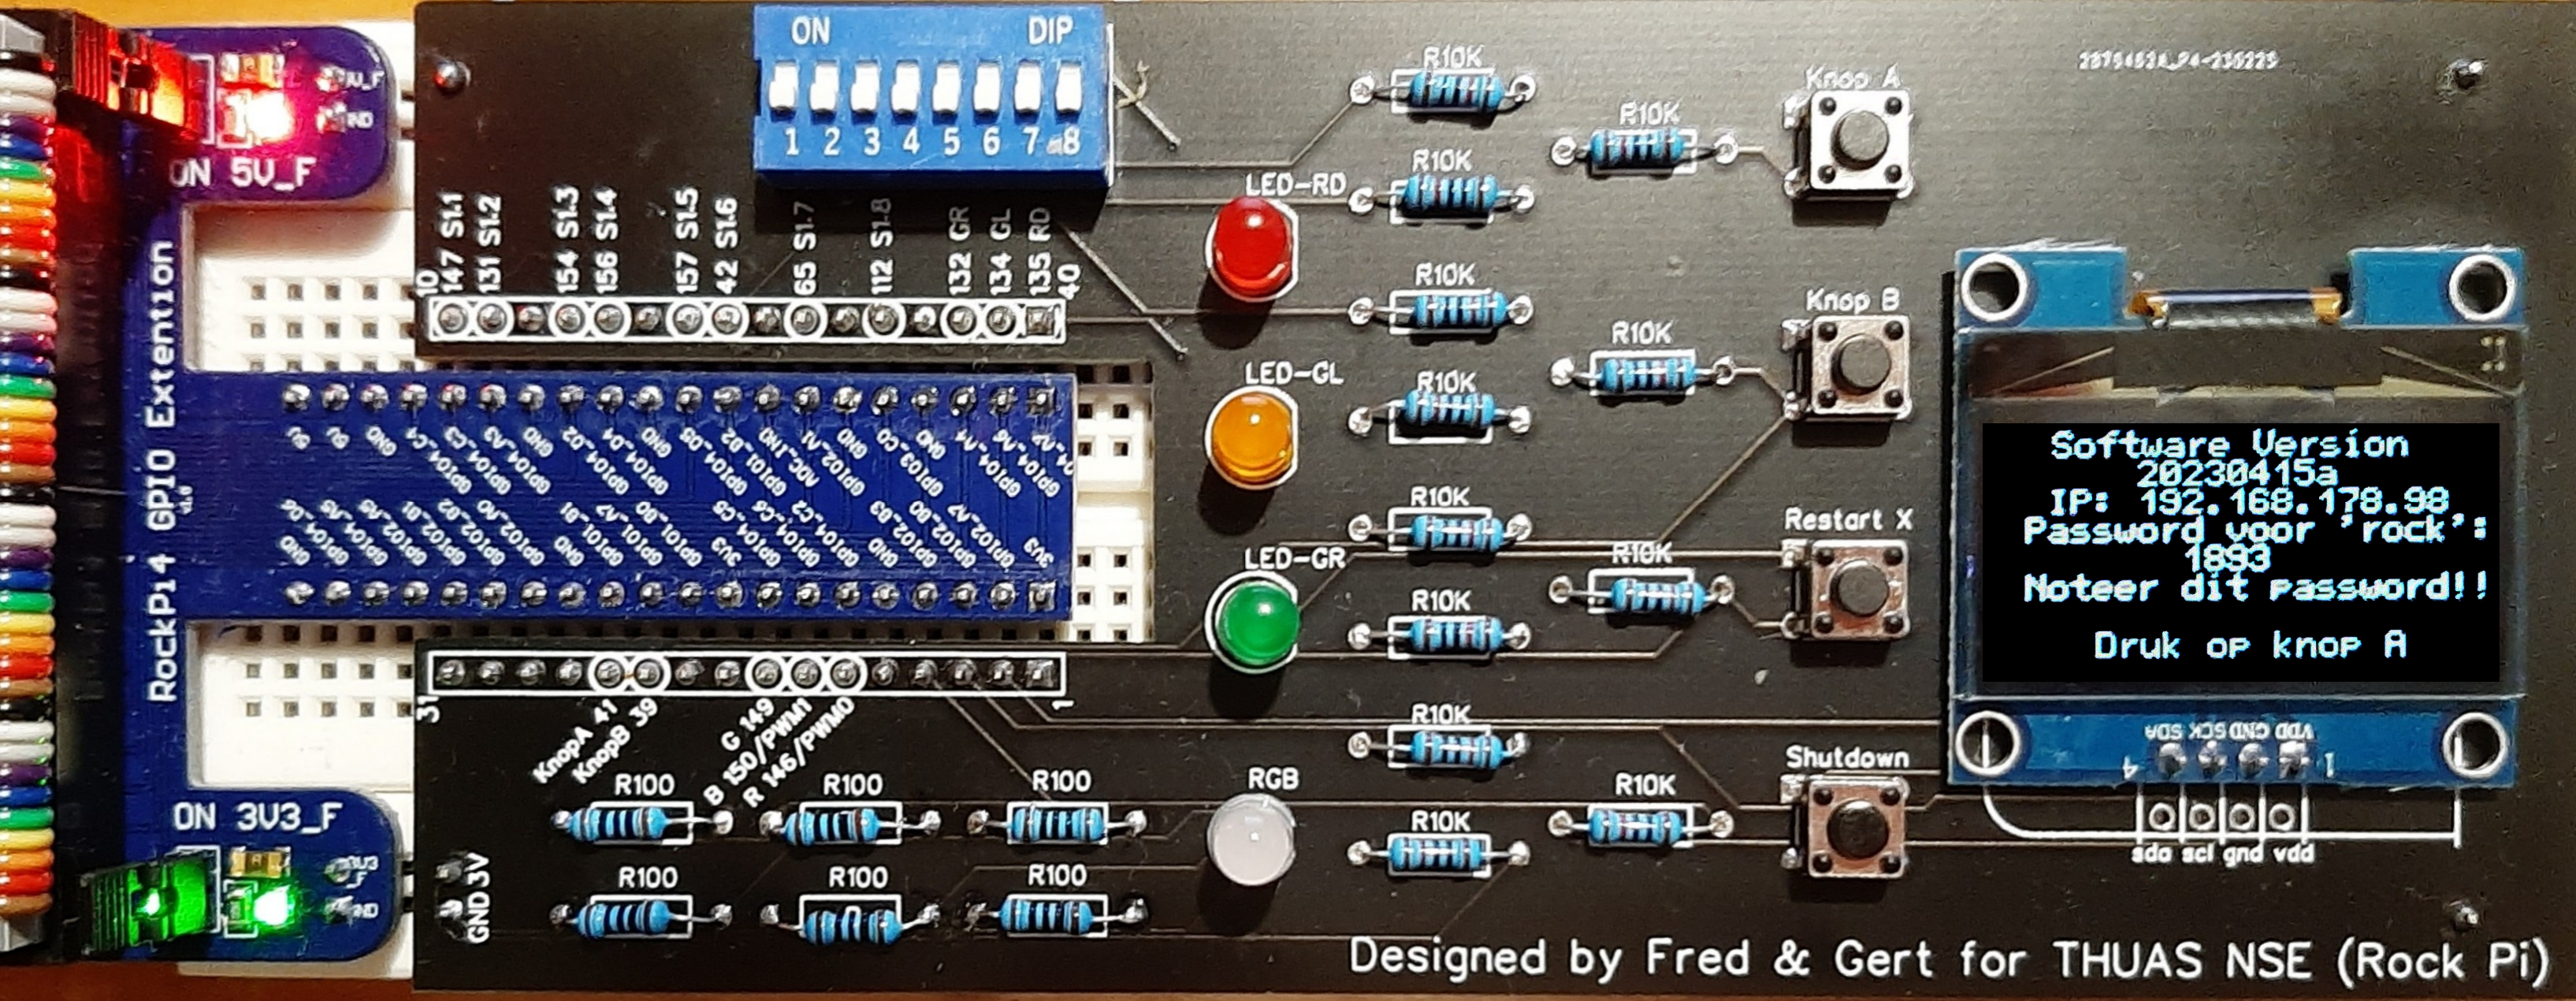
\includegraphics[width=0.62\textwidth]{figuren/rockIPnr}
		\caption{De rockPi met het \textit{IPnr.}}
		\label{fig:rockpiip}   
	\end{center}
\end{figure}
 Het IP nummer van de rockPi is af te lezen via het schermpje, zoals in figuur \ref{fig:rockpiip} wordt weergegeven. In dit voorbeeld is het IP nummer \textit{192.168.1.21}.


Open in windows een terminal (b.v. een powershell, cmd prompt of een extern programma zoals b.v. putty), b.v.powershell. Ga naar windows search, zie figuur \ref{fig:windowsZk} en
\begin{figure}[h!]
	\centering
	\begin{center} 	
		\begin{subfigure}[b]{0.45\textwidth}
			\includegraphics[width=0.95\textwidth]{figuren/windowsPowerShellSearch}
			\caption{Zoekscherm in windows}
			\label{fig:windowsZk}
		\end{subfigure}
		\begin{subfigure}[b]{0.50\textwidth}
			\includegraphics[width=0.95\textwidth]{figuren/powershell}
			\caption{ssh verbinding maken naar de rockPI }
			\label{fig:sshPi}
		\end{subfigure}
		\caption{Opstelling bij opdracht 1.}
		\label{fig:contactPi}   
	\end{center}
\end{figure}
type vervolgen in \textit{powershell}. In de powershell kan het \textit{ssh} commando met de username en ipnr gegeven worden, zoals in figuur \ref{fig:sshPi} wordt weergegeven. Bij de eerste keer zal de melding komen of de host key moet worden opgeslagen, type in\textit{ yes}. Vervolgens zal om om het password gevraagd worden. Dit is \textit{rock}. 

Wanneer het inloggen gelukt is, verschijnt eerst een verhaaltje dat eindigt met de prompt van de rockPI, zoals in figuur \ref{fig:rockpiLogIn} te zien is.
\begin{figure}[h!]
	\centering
	\begin{center} 	
		\includegraphics[width=0.7\textwidth]{figuren/ingelogtRockPi}
		\caption{Ingelogd in de rockPi}
		\label{fig:rockpiLogIn}   
	\end{center}
\end{figure}
Vanaf nu werk je in een linux terminal omgeving. Een listing van een directory kan opgevraagd worden met het \textit{ls} commando, het veranderen van een directory kan gedaan worden het \textit{cd} commando (change directory) en het maken van een directory met het \textit{mkdir}  commando (make directory). Verdere linux commando's en tips zijn te vinden in appendix \ref{app:linux}.



\subsection{Het aansturen van een LED.}


Wanneer contact is gemaakt met de Pi, zoals beschreven in hoofdstuk \ref{chp:contactPi}, kunnen de LEDs aangestuurd worden. De LED's zitten aangesloten op de GPIO (General Purpose Input Output) connector van de RockPI, deze is te zien in figuur \ref{fig:rockpiCon}.
\begin{figure}[h!]
	\centering
	\begin{center} 	
		\includegraphics[width=0.9\textwidth]{figuren/rockpi-connector}
		\caption{De GPIO connector van de RockPI}
		\label{fig:rockpiCon}   
	\end{center}
\end{figure}
De buitenste kolom geeft aan de GPIO nummer die gebruikt kan worden waarop deze geprogrammeerd kan worden. Zo zit de rode LED aangesloten op GPIO nummer 135. \\


\paragraph[Opdracht 1a]{Opdracht 1a, het eerste programmaatje op de RockPI}	

\begin{enumerate}
	\item Plaats de USB stick in de Rock PI.
	\item Ga naar de directory van je USB stick
	\begin{itemize}
		\item \textit{cd /media/rock}
	\end{itemize}
    
    \item Maak een directory \textit{ledje} aan en ga daar na toe.
	\begin{itemize}
	    \item \textit{mkdir ledje}
	    \item \textit{cd ledje}
    \end{itemize}  
   \item Download files \textit{gpiofuncties.h}, \textit{gpiofuncties.cpp}, \textit{test.cpp} van git hup. Het main programma (\textit{test.cpp}) wordt in Listing \ref{lst:mainLd} weergegeven
   	\begin{itemize}
     	\item \textit{git clone https://github.com/JohnVi-hhs/oop.git}
     	
     
  	
   \end{itemize}

\begin{lstlisting}[caption=Zet LED aan en uit,frame=tlrb,label={lst:mainLd}]{Name}
#include <unistd.h>
#include <iostream>
#include "gpiofuncties.h"
	
using namespace std;
#define RODELED 135
	
int main() {
		
	cout<<"Hi NSE"<<endl;
	int b=zetPinOpOutput(RODELED);//return waarde of het gelukt is.
	if(b == 0)  {  //if(!b) mag ook. 
		cout<<"Foutje bedankt"<<endl;
		return 0;
	}
	cout<<"b= "<<b<<endl;//return waarde of het gelukt is.
	b=zetPinWaarde(RODELED,1);  //Zet de rode LED aan.
	usleep(1000000);
	b=zetPinWaarde(RODELED,0);  //Zet de rode LED uit.
	cout<<"einde"<<endl;
}
\end{lstlisting}
   \item Compileer en run het testprogramma.
\begin{itemize}
	\item Compileren van het programma. \\\textit{g++ -g3 *.cpp -o tst}\\
	optie \textit{-g3} heeft te maken met debug mogelijkheden. \\
	Optie \textit{-o} geeft een naam aan de output file (\textit{tst})
	\item Voer het zojuist gecompileerde programma tst uit.\\\textit{./tst}  
	
\end{itemize}
Resultaat:\\	
De rode LED gaat 1 seconde aan.

\item Pas het programma zodanig aan, zodat eerst de groene LED aangaat, daarna de gele LED en vervolgens de rode LED. \\
In de linux terminal, kunnen verschillende editors gebruikt worden, waarvan \href{https://linuxize.com/post/how-to-use-nano-text-editor/}{nano} \'{e}\'{e}n van de meest gebruikte is, een ander beroemde/beruchte editor is \href{https://opensource.com/article/19/3/getting-started-vim}{vim}  

\end{enumerate}

\section{Het werken vanuit Visual Studio Code}

Hierbij wordt vanuit Visual Studio Code (VSC) gewerkt, en wordt de klasse Led geïmplementeerd. Er wordt vanuit gegaan dat VSC geïnstalleerd is, zoals in appendix  \ref{app:vsc} beschreven staat.  
\begin{enumerate}
	\item Start VSC op en maak verbinding met de RockPi.
	\begin{itemize}
		\item Klik op remote Explorer \img{figuren/remoteExplorer}. De IP nummers van de remote system(en) die al eerder gebruikt zijn worden zichtbaar, zoals te zien is in Figuur \ref{fig:remNr}
		\begin{figure}[h!]
			\centering
			\begin{center} 	
				\includegraphics[width=0.5\textwidth]{figuren/remoteExplorer2}
				\caption{Remote Explorer van VSC}
				\label{fig:remNr}   
			\end{center}
		\end{figure}
				 
		\item  Maak een nieuwe connectie aan, door op \img{figuren/connectIcon} te klikken.

      \end{itemize}
      
      \item Nadat een verbinding gemaakt is met de RockPi, open een remote folder door op \img{figuren/VSCiconeExpl} te klikken of (Cntrl + k Cntrl + o) en ga naar de directory van de vorige opdracht. Aan de linkerkant worden de files zichtbaar en onderaan een statusbalk met informatie, indien de runnable extensie \img{figuren/runnableExt} geïnstalleerd is. Dit is te zien in figuur \ref{fig:vncOp}
  		\begin{figure}[h!]
  	\centering
  	\begin{center} 	
  		\includegraphics[width=0.5\textwidth]{figuren/vncSchermOp1}
  		\caption{VSCode in de gewenste directory}
  		\label{fig:vncOp}   
  	\end{center}
  \end{figure}    

Klik op select folder  en selecteer de folder waarin de files staan. Hierna voert de Runnable extensie een aantal opdrachten uit en wordt de statusbalk uitgebreid, zoals te zien is in figuur \ref{fig:vncstsblk}.
  		\begin{figure}[h!]
	\centering
	\begin{center} 	
		\includegraphics[width=0.5\textwidth]{figuren/statusbalk2}
		\caption{De statusbalk nadat de directory is gekozen.}
		\label{fig:vncstsblk}   
	\end{center}
\end{figure} 

Klik op \img{figuren/vncComp} , de runnable extension compileert nu het programma.
\item Door met de debugger te werken, kan een aantal onduidelijkheden van het programmeren verduidelijkt worden.
\begin{itemize}
	\item Klik links van regelnummer 10, er verschijnt een rode stip, dit is een breakpoint.
	\item Klik op \img{figuren/startDebug}, de debugger wordt gestart en het  beeldscherm zoals in figuur \ref{fig:debugScherm} verschijnt.
	\begin{figure}[h!]
		\centering
		\begin{center} 	
			\includegraphics[width=0.5\textwidth]{figuren/debugScherm}
			\caption{Start van de debug sessie.}
			\label{fig:debugScherm}   
		\end{center}
	\end{figure}
	
	Met de debugknoppen rechtsboven kan nu stap voor stap door het programma gelopen worden.\\
	Doorloop het programma stap voor stap, zodat de LED ook daadwerkelijk bij een stap aan- en uitgaat. 
\end{itemize}

\item Bij deze opdracht wordt de eerst klasse gemaakt.
\begin{itemize}
	\item Maak een nieuwe terminal aan (Terminal $\rightarrow$ New Terminal) of Cntr +Shift+` en maak een nieuwe directory aan.
	\item clone de volgende code:\\
	 git clone \verb|--|branch opdrLedH https://github.com/JohnVi-hhs/oop.git
	\item De klasse \textbf{Led} wordt weergegeven in figuur \ref{fig:klassLed}
		\begin{figure}[h!]
		\centering
		\begin{center} 	
			\includegraphics[width=0.37\textwidth]{figuren/klasseLedOpg1}
			\caption{Diagram van de klasse Led}
			\label{fig:klassLed}   
		\end{center}
	\end{figure}
	
	Implementeer de Led.cpp
	
\end{itemize}


    \end{enumerate}


\section{Het werken met een visuele debugger.}
 
Bij dit onderdeel van de opdracht wordt gewerkt met een grafische debugger. Hiermee wordt een grafische weergave gedaan wat een object is en wat een object van een afgeleide klasse inhoud (dit laatste komt in opgave 3 te spraken). Verder worden de associaties tussen objecten duidelijk weergegeven (dit wordt in week 4 en 5 gedaan).

De grafische debugger die gebruikt wordt is de DDD debugger(Data Display Debugger) 


Een paar handige links hierbij zijn:

\begin{itemize}
	\item DDD manual in \href{https://www.gnu.org/software/ddd/manual/html_mono/ddd.html}{html} en \href{https://www.gnu.org/software/ddd/manual/pdf/ddd.pdf}{pdf}
	\item \href{https://www.gnu.org/software/ddd/}{GNU DDD project}
	\item \href{href="https://taufanlubis.wordpress.com/2019/02/19/gnu-debugger-front-end-graphical-user-interface-with-ddd}{taufanlubis.wordpress.com}
	\item  \href{https://www.cs.swarthmore.edu/~newhall/unixhelp/howto_gdb.php}{Swarthmore}
	\item  \href{http://www.linuxfocus.org/English/January1998/article20.html}{linuxfocus}
\end{itemize}

De instellingen van de DDD debugger staan in de file .ddd die staat in de home directory (\textit{/home/rock}). Soms is het eenvoudiger om deze directory te deleten dan de instellingen aan te passen.

We gaan nu met de DDD debugger werken.
Om met DDD te kunnen werken hebben we een grafische omgeving nodig. Een handige methode is om de de VNC viewer van de host te gebruiken. Deze viewer toont de grafische uitvoer van de RockPi. Open in de VNC een terminal, ga naar de directory die in de opdracht \ref{en:dir} van hoofdstuk \ref{hfst:strt}  aangemaakt is (waar de files blink1.cpp, Led.cpp en Led.h \textcolor{green}{blink1} staan) en start de DDD debugger op:
\texttt{\textit{ddd blink1}}, vervolgens wordt het scherm, zoals weergegeven in Figuur \ref{fig:dddscherm1}, getoond.
\begin{figure}[h!]
	\captionsetup{justification=centering}
	\includegraphics[width=0.7 \linewidth]{figuren/ddd_startup_screen}
	\centering
	\caption{het DDD opstartscherm.}
	\label{fig:dddscherm1}
\end{figure}

\paragraph{Opdracht}
We gaan hierbij stap voor stap het programma doorlopen, waarbij de inhoud van de objecten van de klasse Led wordt getoond.

\begin{enumerate} [label=\alph*]
	\item Als eerste een korte kennismaking met de DDD debugger.
\begin{enumerate} [label=\roman*]

	\item Ga met de cursor op de regel \texttt{\textit{ Led ld1(18, "Pietje Puk");}}
	(regelnummer 22)
	\item Klik op \textit{Break} (bij algemene commando's). Voor het begin van de regel verschijnt nu een breakpoint.

\begin{figure}[h!]
	\captionsetup{justification=centering}
	\includegraphics[width=0.7 \linewidth]{figuren/ddd_set_breakpoint}
	\centering
	\caption{het zetten van een breakpoint.}
	\label{fig:ddduitv1}
\end{figure}
	\item Klik op \textit{Run} (bij debug commando's),
het programma wordt uitgevoerd tot het breakpoint. Er verschijn een groene pijl bij het breakpoint.
\item Klik op \textit{Next}, de regel wordt uitgevoerd. \\
De groene pijl komt voor de regel \textit{Led ld2(23);} te staan. 
\item Klik op step, met dit commando \textit{Step} wordt in de constructor van de klasse Led gestapt. Doorloop het programma verder stap voor stap.

\end{enumerate}
\item Het zichtbaar maken van de inhoud van de objecten.


\begin{enumerate} [label=\roman*]
	\item Start de DDD debugger op (\texttt{\textit{ddd blink1}}):
		\item Zet een breakpoint op de regel	\textit{ld1.zetAan();} 
		\item Klik met de muis op variabele \texttt{ld1} en vervolgens op Display of klik met rechtermuisknop en vervolgens op Display ld1.
		\item Doe hetzelfde met variabele \textit{ld2}. 
		\item Als het goed is ziet de debugger er ongeveer uit zoals Figuur \ref{fig:dddLeds}, alleen met je \textcolor{BrickRed}{eigen naam}.  
	    \item Ga met het Step commando de methode \texttt{zetAan} van l1 in.
		\item Ga met het Step commando de methode \texttt{zetAan} van l2 in. Je ziet dat de methode hetzelfde is, alleen de attributen hebben een andere waarde.
		  \begin{figure}[h!]
		 	\captionsetup{justification=centering}
		 	\includegraphics[width=0.9 \linewidth]{figuren/LedDDD}
		 	\centering
		 	\caption{Weergave van twee objecten van de klasse Led.}
		 	\label{fig:dddLeds}
		 \end{figure}
\end{enumerate}
	 \item Maak een screenshot die lijkt op Figuur \ref{fig:dddLeds} alleen met je \textbf{eigen naam} in plaats van "Pietje Puk" en upload deze op Brightspace.
	 \item Laat de opdracht aftekenen met onder andere een zichtbaar screenshot.
 
\end{enumerate}


%	\input{rockopdracht2}
	
	\input{appendix}
	\begin{comment}
	\maketitle
	
	
	\tableofcontents
	
	\let\cleardoublepage\clearpage
	\let\cleardoublepage\clearpage
	
	
%	\chapter{Inleiding}\label{chap:inl}
Voor het practicum OOPR1 zijn (ongeveer) 25 RockPi’s beschikbaar. Dit zijn Raspberry Pi achtige ‘Single Board Computers’ die met een Linux variant werken, in dit geval Debian 10. De RockPi’s zijn aangeschaft omdat Raspberry Pi’s niet leverbaar (of te duur) waren.
Tijdens het practicum gebruik je een RockPi van school. Je kunt deze alleen op school gebruiken, je mag hem niet meenemen naar huis. Dat is dan ook het belangrijkste nadeel.

Het gebruik van de RockPi heeft een aantal voordelen:
\begin{itemize}
\item Je hoeft zelf niets aan te schaffen
\item Je werkt onder gecontroleerde omstandigheden: de verstrekte RockPi bevat alles wat nodig is voor het practicum. Dat betekent dat jij- of de docent niet eerst moet puzzelen om de omgeving aan de praat te krijgen.
\end{itemize}

\hypertarget{USBinleiding}{}
Bij het practicum heb je \textit{je eigen} USB stick nodig om je bestanden op te zetten (\textit{geen gedeelde!}). Een USB stick van 1GB is goed genoeg (128+ MB). Groter mag, maar is zinloos.
\begin{itemize}
\item Je werkt op je eigen \hyperlink{chp:USBstick}{USB stick} en niet op het bestandssysteem van de RockPi. 
\item Na afloop van het practicum lever je de RockPi in zonder daar bestanden op achter te laten. 
\item Ga er vanuit dat de RockPi’s na een practicum gewist worden!
\end{itemize}

\section{Voorbereiding - Software installeren}
Zorg dat je vóór het practicum de benodigde software geïnstalleerd hebt.
Zie Bijlage \ref{app:instal} voor software installatie.
\newpage

\begin{comment}
\begin{itemize}
\item Installeer Github Desktop: \url{https://desktop.github.com/}
\item Vanuit Github Desktop, druk Ctrl+Shift+O voor 'Clone repository' en voeg de repository \textbf{JohnVi-hhs/oop} toe.
\item Installeer 'Visual Studio Code' (VSC) volgens de instructies in \newline \url{https://github.com/Grrtzm/OOPR1} \textit{(moet nog aangepast worden)}
\item Download en installeer de VNC viewer:  \newline \url{https://www.realVNC.com/en/connect/download/combined/}
\item (Optioneel maar wel handig) Download en installeer de SSH client KiTTY  \newline \url{https://www.fosshub.com/KiTTY.html} \newline
KiTTY is een opvolger van PuTTY. Het grote voordeel is dat KiTTY automatisch opnieuw verbinding maakt als de verbinding even verbroken is geweest.
\end{itemize}
\end{comment}

\section{Eerste gebruik van de RockPi}
We gaan er van uit dat je de RockPi in lokaal D2.001 of D2.003 van HHS Delft gebruikt. \newline
De RockPi is al ingesteld voor Wi-Fi netwerk in D2.001: \textbf{Lab001}. \newline
Log ook met je laptop in op dit netwerk. Het password is \textbf{Lab001WiFi}. \newline
In Figuur \ref{fig:netw} wordt weergegeven hoe de RockPi op het lab netwerk is aangesloten.
\begin{figure}[h!]
	\centering
	\begin{center} 	
		\includegraphics[width=0.4\textwidth]{figuren/laBnetwork}
		\caption{De RockPi in het lab netwerk}
		\label{fig:netw}   
	\end{center}
\end{figure}
\break
Sluit de USB-C voedingskabel aan zodat de RockPi gaat opstarten (op de RockPi gaat een groene led branden). Verder hoef je nog niets aan te sluiten!
\begin{figure}[h!]
	\centering
	\begin{center} 	
		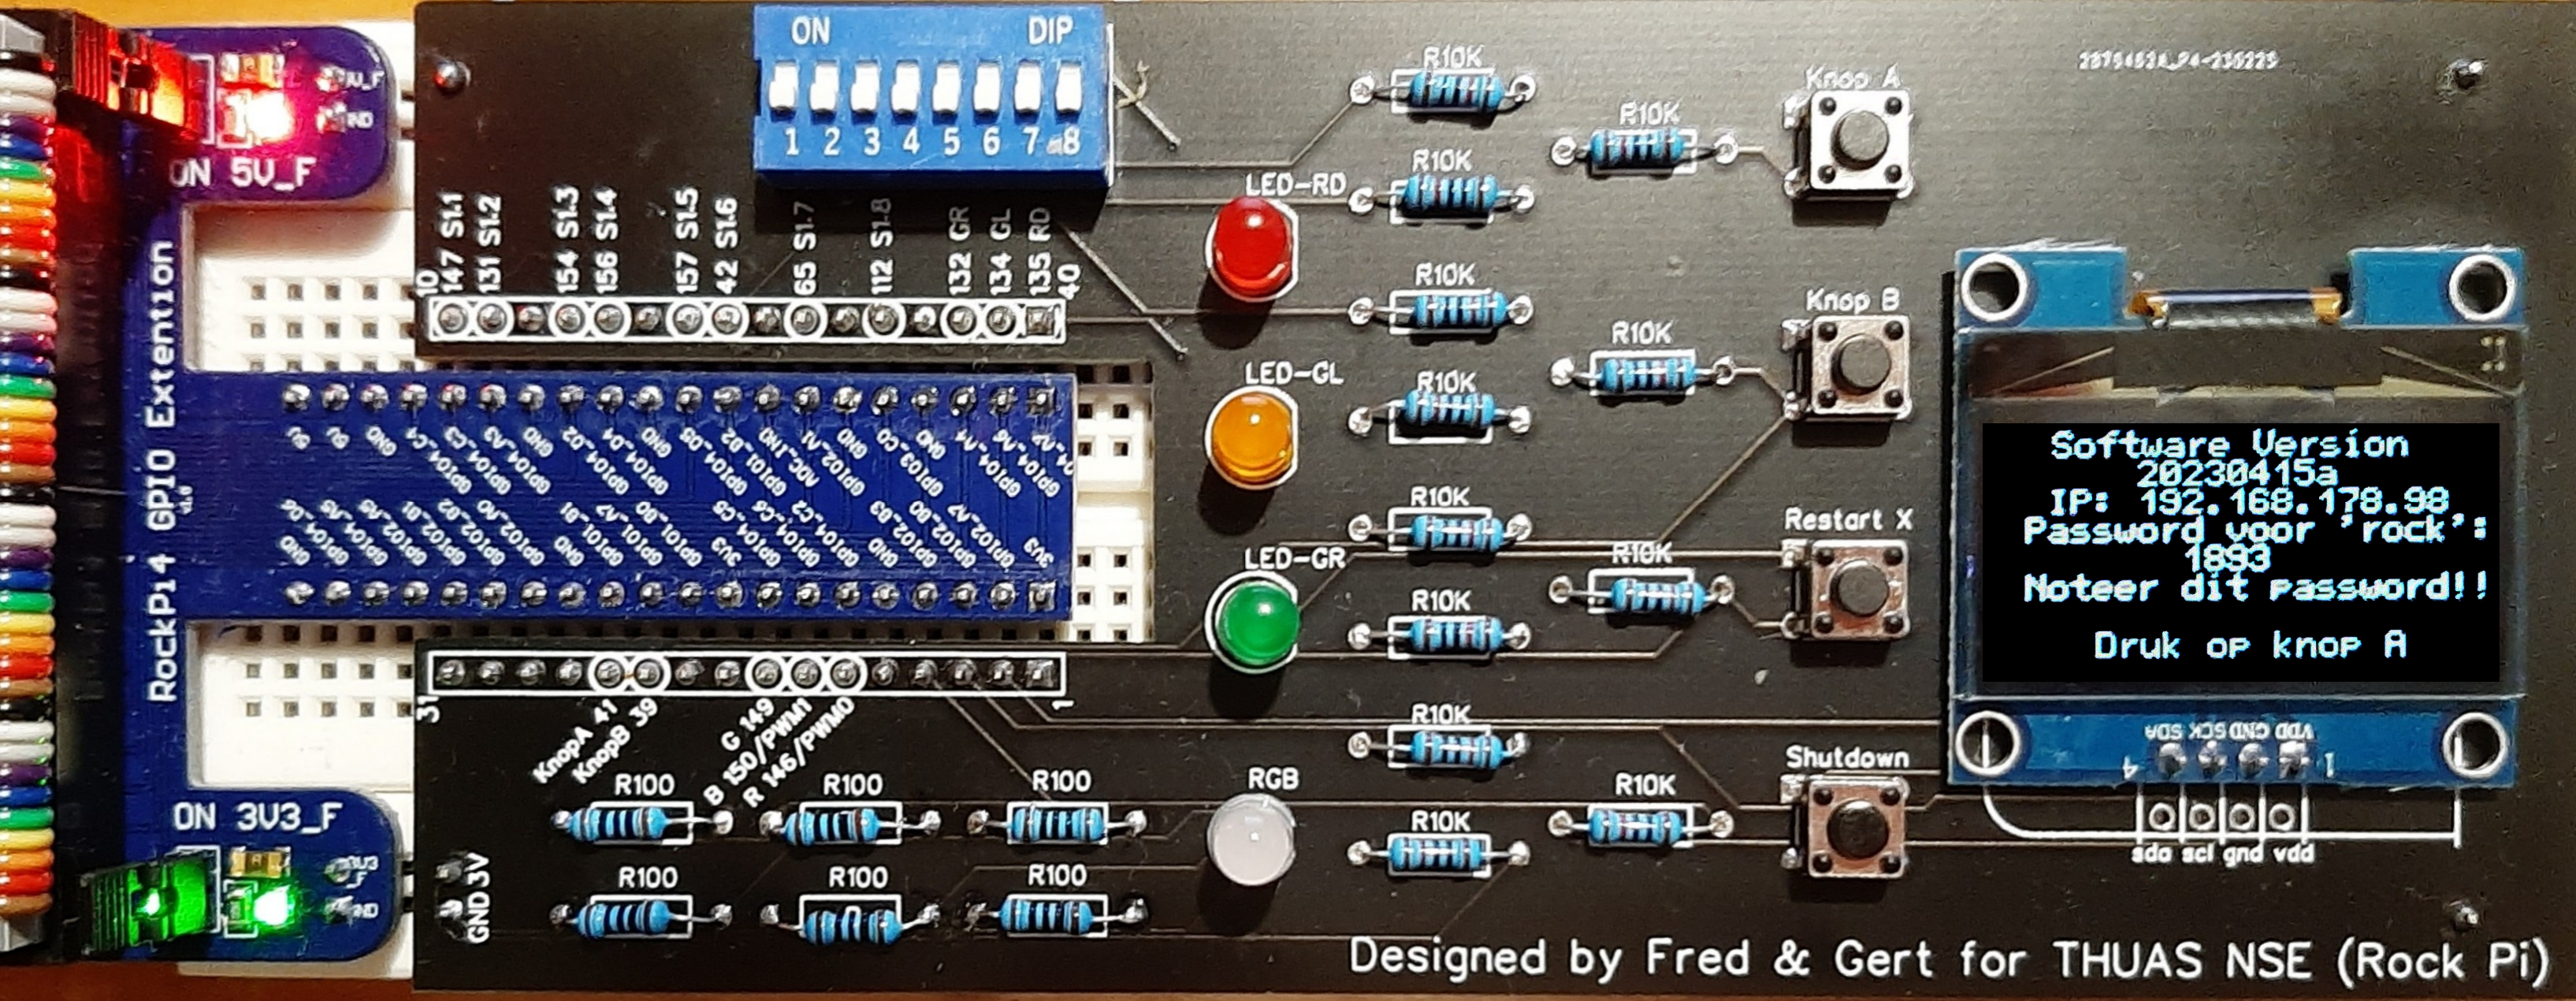
\includegraphics[width=1\textwidth]{figuren/rockIPnr}
		\caption{Het uitbreidingsbord van de RockPi}
		\label{fig:rockIPnr}   
	\end{center}
\end{figure}

\textbf{\textit{Controleer de zelftest:}} Om zeker te weten dat het bovenstaande bordje OK is gaat de RockPi alle leds even aan en uitzetten. \newline
Als je de RockPi in het lab (D2.001) aanzet, verschijnt op het oled display bij “IP address for wlan0:” een IP adres van het Lab001 Wi-Fi netwerk (zie Figuur \ref{fig:rockIPnr}). \newline
Nu kun je via SSH en/of VNC een verbinding maken met dit IP adres en inloggen op de RockPi.
De username is \textbf{rock}, het password is ook \textbf{rock}. Mocht er een sudo password gevraagd worden, dan is dit ook \textbf{rock}.
Overigens kun je ook een ethernet kabel aansluiten zoals in Figuur \ref{fig:rockIPnr} te zien is bij “IP address for eth0:”.\break\newline
Zorg wel dat je PC op hetzelfde netwerk is aangesloten. Als VNC het niet wil doen, maar ssh wel, dan zitten je PC en de RockPi mogelijk op verschillende Wi-Fi access-points. Als VNC niet werkt, maar je RockPi en laptop zitten wel op hetzelfde netwerk, dan kun je het knopje '\textbf{Restart\_X}' indrukken, dit herstart de grafische schil op de RockPi.

Zodra je bent ingelogd met VNC, kun je je USB stick aansluiten en configureren. Het maakt niet uit welke USB poort je gebruikt. 

Als je klaar bent met je practicum, moet je de RockPi netjes afsluiten. Door op het knopje ‘\textbf{Shutdown}’ te drukken, wordt het operating system netjes afgesloten zodat het bestandssysteem niet corrupt raakt (wat kan gebeuren als je de RockPi gewoon uitzet).

'Knop\_A' kun je gebruiken om tijdens het opstarten voor volledig GPIO gebruik te kiezen; druk de knop in vóórdat je de RockPi aanzet, en houd hem ingedrukt tot de LED zelftest klaar is. Dit is zo gedaan omdat wisselen tussen PWM gebruik (voor de rode en blauwe leds van de driekleuren led) en GPIO (alleen aan en uit, geen ‘analoge’ waarden) niet lukt zonder opnieuw op te starten.

Aan 'Knop\_A', 'Knop\_B' en de DIP switches (blauwe blokje) zijn verder geen functies toegewezen. Daar kun je zelf code voor schrijven.

\section{Inloggen met VNC}
Controleer even of het werkt. Je gaat dit later pas gebruiken. \\Voer het IP adres zoals getoond op het oled display in op VNC (Figuur \ref{fig:rockIPnr}).\newline
Log in op de RockPi en klik op het ‘Terminal’ icoon (rood omcirkeld in Figuur \ref{fig:termico}):
\begin{figure}[h!]
	\centering
	\begin{center} 	
		\includegraphics[width=0.4\textwidth]{figuren/Terminal-icoon}
		\caption{Terminal icoon}
		\label{fig:termico}   
	\end{center}
\end{figure}

Nu verschijnt het Terminal venster. Van hieruit kun je allerlei commando's invoeren (en tegelijk wordt o.a. schermresolutie ingesteld en wordt de screensaver uitgezet):
\begin{figure}[h!]
	\centering
	\begin{center} 
		\includegraphics[width=0.9\textwidth]{figuren/terminal-inlogscherm}	
		\caption{Het Terminal scherm}
		\label{fig:terminal-inlogscherm}   
	\end{center}
\end{figure}

\hypertarget{chp:USBstick}{}
\section{USB Stick voorbereiden}
\textbf{\textit{LET OP!! }}
\begin{itemize}
	\item Met onderstaande procedure verwijder je alle bestanden van je USB stick!
	\item Je hebt genoeg aan een \hyperlink{USBinleiding}{kleine USB stick} (ergens tussen 128MB en 4 GB).
	\item Je kunt hierna alléén met Linux op je USB stick kijken, niet meer met Windows!
\end{itemize}

Formatteer nu je USB stick met EXT4 filesystem. Dit is nodig omdat Linux d.m.v. attributen in het bestandssysteem aangeeft of een bestand uitvoerbaar (‘executable’) is. Dat is op  een Windows compatible USB stick (met FAT of NTFS bestandsysteem) niet mogelijk.
Kijk of je USB stick gezien wordt. Geef het commando \textbf{\texttt{lsblk}} en kijk of daar een device bij zit met sda in de naam (zie hieronder in de listing van \texttt{lsblk}). In dit geval is deze er. De partitie waar we gebruik van maken is /dev/sda1.

\begin{lstlisting}[language=bash]
rock@rockpi-4b:~$ lsblk
NAME         MAJ:MIN RM   SIZE RO TYPE MOUNTPOINT
sda            8:0    1   1.9G  0 disk
`-sda1         8:1    1   1.9G  0 part /media/rock/9C02-C2F1
mmcblk1      179:0    0 115.2G  0 disk
|-mmcblk1p1  179:1    0   3.9M  0 part
|-mmcblk1p2  179:2    0     4M  0 part
|-mmcblk1p3  179:3    0     4M  0 part
|-mmcblk1p4  179:4    0   512M  0 part
`-mmcblk1p5  179:5    0   7.8G  0 part /
mmcblk1boot0 179:32   0     4M  1 disk
mmcblk1boot1 179:64   0     4M  1 disk
mmcblk1rpmb  179:96   0     4M  0 disk
}
\end{lstlisting}
	
\underline{\textbf{Controle:}}\newline 
Als je het commando \href{https://www.techrepublic.com/article/linux-101-what-is-the-mount-command-and-how-do-you-use-it/}{\textbf{\texttt{mount}}} geeft, dan verwacht je in de uitvoer het device (de disk) /dev/sda1 te zien: % \textbf{\texttt{mount}}
\begin{lstlisting}
/dev/sda1 on /media/rock/9C02-C2F1 type vfat (rw,nosuid,nodev,relatime,uid=1000,gid=1000,fmask=0022,dmask=0022,codepage=936,iocharset=utf8,shortname=mixed,showexec,utf8,flush,errors=remount-ro,uhelper=udisks2)
\end{lstlisting}

Hierboven zie je dat disk ge-'mount' is. Om te formatteren moet je eerst 'umount' doen:\newline
\textbf{\texttt{umount /dev/sda1 }}\newline
Nu USB disk formatteren met ext4 filesystem (sudo password is \textit{rock}):\newline
\textbf{\texttt{sudo mkfs -t ext4 /dev/sda}}\newline
Vervolgens disklabel 'Documents' instellen:\newline
\textbf{\texttt{sudo e2label /dev/sda Documents}}\newline
Als laatste gebruiker \textit{rock} eigenaar maken van de USB stick:\newline
\textbf{\texttt{sudo chown rock /home/rock/Documents}}\newline

Hieronder zie je de output van bovenstaande commando's:
	
\begin{lstlisting}[language=C]   % Gert: Is het niet, maar hiermee doet hij geen speciale opmaak
rock@rockpi-4b:~\$ umount /dev/sda
umount: /dev/sda#: No such file or directory
rock@rockpi-4b:~\$ sudo mkfs -t ext4 /dev/sda
mke2fs 1.44.5 (15-Dec-2018)
/dev/sda contains a vfat file system
Proceed anyway? (y,N) y
Creating filesystem with 491520 4k blocks and 123120 inodes
Filesystem UUID: 1b2275ec-6dbd-4f3b-8d41-feaf4da0c7b7
Superblock backups stored on blocks:
32768, 98304, 163840, 229376, 294912

Allocating group tables: done
Writing inode tables: done
Creating journal (8192 blocks): done
Writing superblocks and filesystem accounting information: done
\end{lstlisting}

Als het formatteren en labelen klaar is, kun je testen of de USB stick correct gezien wordt:\newline
Verwijder de USB stick, wacht even en steek hem weer terug in een USB poort.\newline
Klik in VNC op het ‘File Manager’ icoon (rood omcirkeld in Figuur \ref{fig:fileman}):

\begin{figure}[h!]
	\centering
	\begin{center} 	
		\includegraphics[width=0.4\textwidth]{figuren/File-Manager}
		\caption{Terminal icoon}
		\label{fig:fileman}   
	\end{center}
\end{figure}
Ga in de ‘File Manager’ naar het ‘Documents’ device.\newline
Als dit werkt, dan zie je onderin de statusbalk van de ‘File Manager’ hoeveel vrije ruimte je USB stick heeft (rood omcirkeld in Figuur \ref{fig:fileman})

\begin{figure}[h!]
	\centering
	\begin{center} 	
		\includegraphics[width=1\textwidth]{figuren/FileManagerUsbStick}
		\caption{File Manager}
		\label{fig:FileManagerUsbStick}   
	\end{center}
\end{figure}

Met de 'File Manager' kun je in het bestandssysteem van Linux kijken.\newline
Bij het practicum begin je altijd in de home directory van gebruiker \textbf{rock} (\texttt{/home/rock}). Je werkt \textit{uitsluitend} in de map Documents (\texttt{/home/rock}).\newline
Als je meer wilt weten over het Linux bestandssysteem, \href{https://www.techrepublic.com/article/linux-101-demystifying-the-linux-directory-structure/}{klik dan hier}.

	\let\cleardoublepage\relax
%	\input{mbed}
\chapter{Klasse en objecten in C++}
Als eerste wordt er contact gelegd tussen de laptop en de RockPi, waarna een LEDje aan- en uitgezet wordt. Vervolgens wordt door middel van een programma een aantal LEDs aangestuurd.


Het practicum wordt gedaan op een RockPi dit is een single board computer dat draait in ons geval met het linux operating systeem. Met behulp van de RockPi wordt tijdens het practicum door middel van objecten diverse LEDs aangestuurd. Dit wordt gedaan door een 1 of een 0 naar naar een file te schrijven. In Figuur \ref{fig:netw} wordt weergegeven hoe de RockPi op het lab netwerk is aangesloten.
\begin{figure}[h!]
	\centering
	\begin{center} 	
			\includegraphics[width=0.4\textwidth]{figuren/laBnetwork}
			\caption{De rockPi in het lab-netwerk}
      	\label{fig:netw}   
	\end{center}
\end{figure}
Dit kan via de lab-wifi of via een UTP kabel. Het bijbehorende Ipnr. wordt getoond op het 
displaytje dat aangesloten is op de RockPi. Om contact te kunnen maken tussen de laptop en de RockPi moet de laptop \textbf{ook} op het \textbf{labnetwerk(Lab001) aangesloten} zijn, b.v. via de wifi.


\section{De eerste kennismaking met de RockPi.}


\subsection{Contact maken met de RockPi}\label{chp:contactPi}

In eerste instantie wordt er contact gemaakt met de RockPi via het \textit{ssh} commando.
\begin{figure}[h!]
	\centering
	\begin{center} 	
		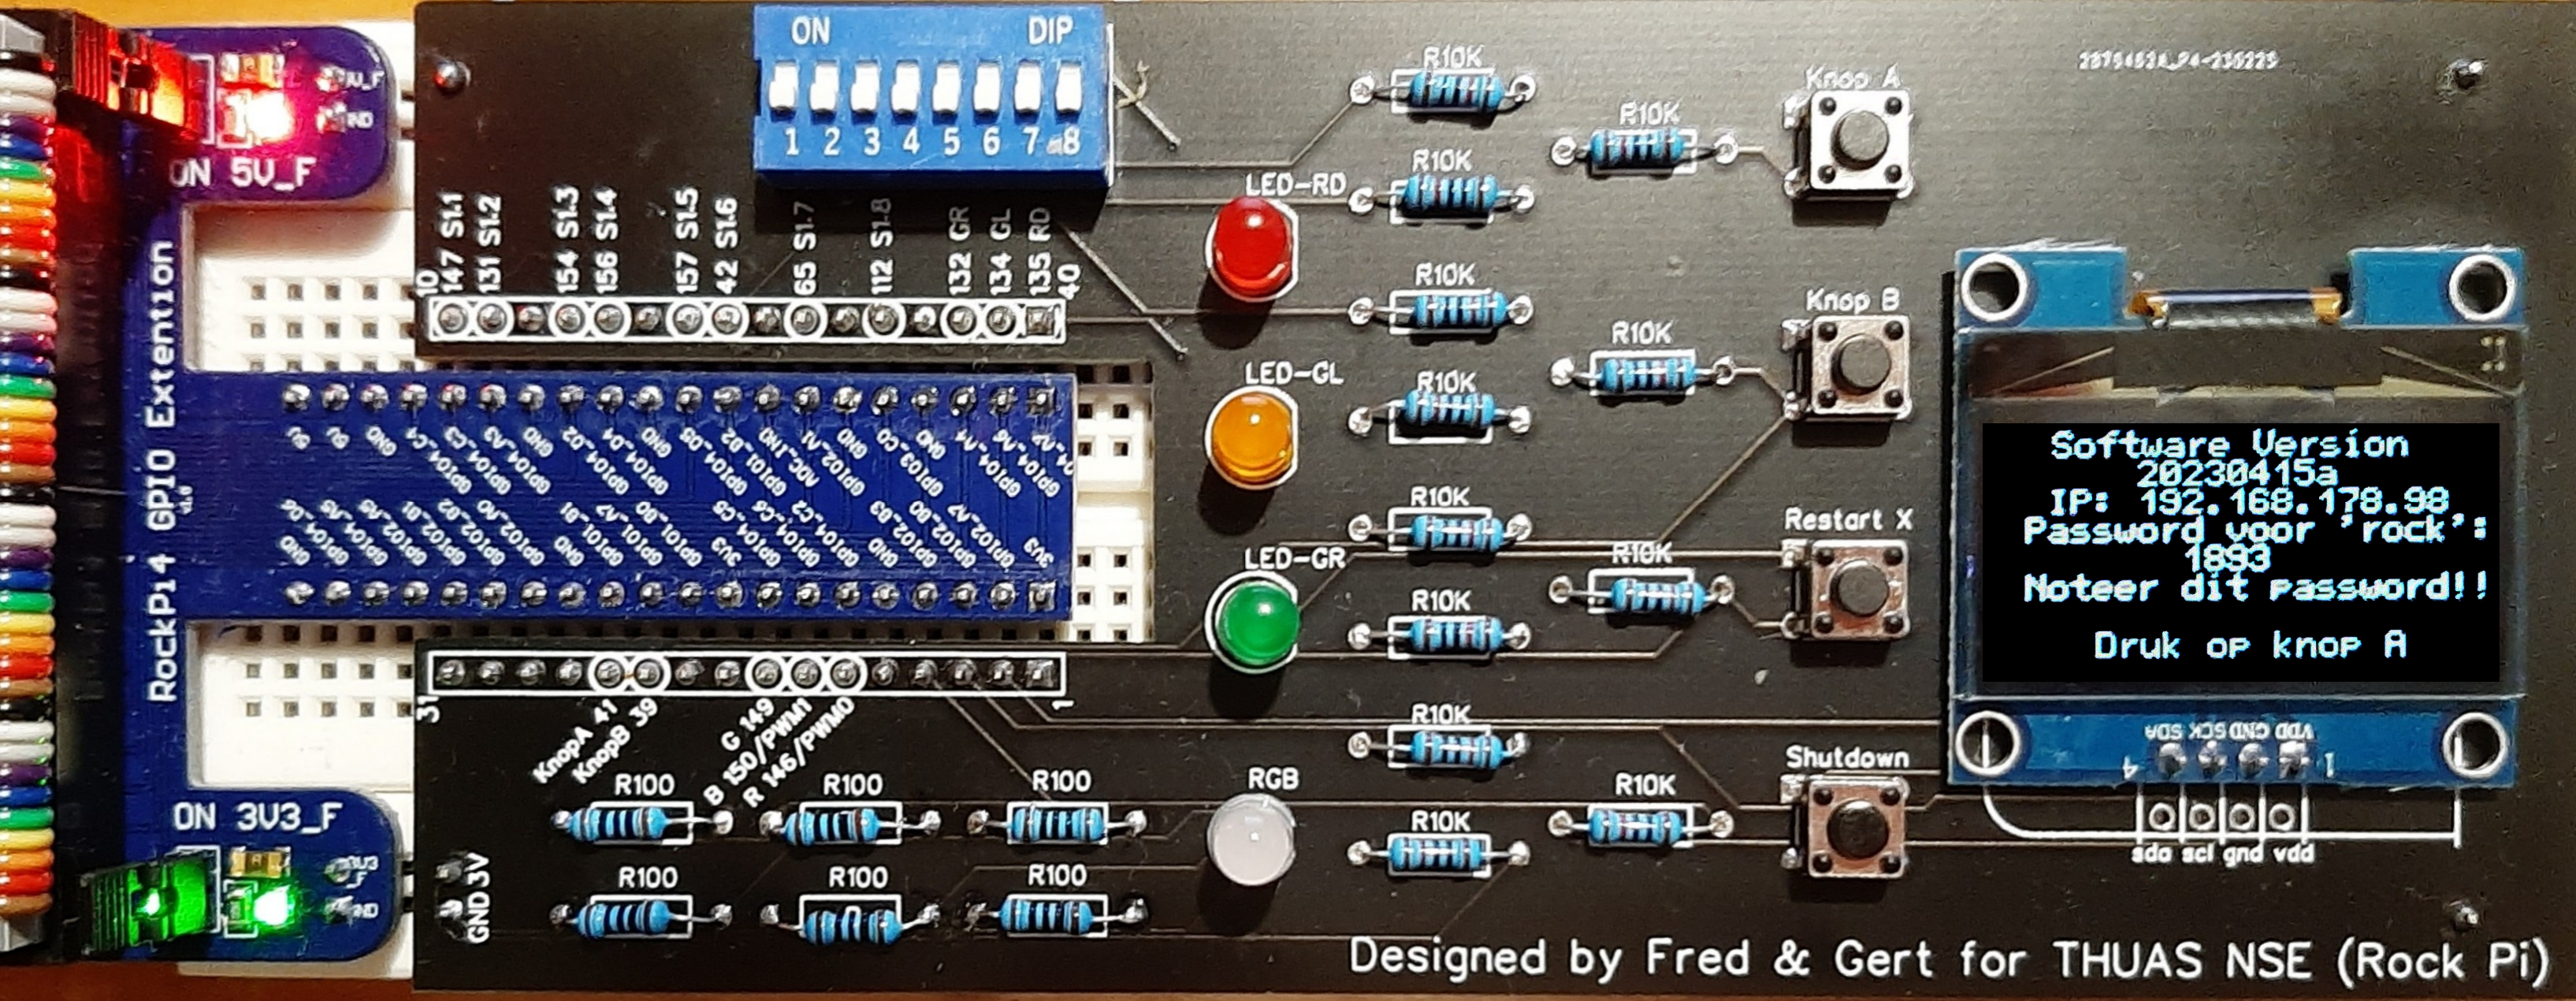
\includegraphics[width=0.62\textwidth]{figuren/rockIPnr}
		\caption{De rockPi met het \textit{IPnr.}}
		\label{fig:rockpiip}   
	\end{center}
\end{figure}
 Het IP nummer van de rockPi is af te lezen via het schermpje, zoals in figuur \ref{fig:rockpiip} wordt weergegeven. In dit voorbeeld is het IP nummer \textit{192.168.1.21}.


Open in windows een terminal (b.v. een powershell, cmd prompt of een extern programma zoals b.v. putty), b.v.powershell. Ga naar windows search, zie figuur \ref{fig:windowsZk} en
\begin{figure}[h!]
	\centering
	\begin{center} 	
		\begin{subfigure}[b]{0.45\textwidth}
			\includegraphics[width=0.95\textwidth]{figuren/windowsPowerShellSearch}
			\caption{Zoekscherm in windows}
			\label{fig:windowsZk}
		\end{subfigure}
		\begin{subfigure}[b]{0.50\textwidth}
			\includegraphics[width=0.95\textwidth]{figuren/powershell}
			\caption{ssh verbinding maken naar de rockPI }
			\label{fig:sshPi}
		\end{subfigure}
		\caption{Opstelling bij opdracht 1.}
		\label{fig:contactPi}   
	\end{center}
\end{figure}
type vervolgen in \textit{powershell}. In de powershell kan het \textit{ssh} commando met de username en ipnr gegeven worden, zoals in figuur \ref{fig:sshPi} wordt weergegeven. Bij de eerste keer zal de melding komen of de host key moet worden opgeslagen, type in\textit{ yes}. Vervolgens zal om om het password gevraagd worden. Dit is \textit{rock}. 

Wanneer het inloggen gelukt is, verschijnt eerst een verhaaltje dat eindigt met de prompt van de rockPI, zoals in figuur \ref{fig:rockpiLogIn} te zien is.
\begin{figure}[h!]
	\centering
	\begin{center} 	
		\includegraphics[width=0.7\textwidth]{figuren/ingelogtRockPi}
		\caption{Ingelogd in de rockPi}
		\label{fig:rockpiLogIn}   
	\end{center}
\end{figure}
Vanaf nu werk je in een linux terminal omgeving. Een listing van een directory kan opgevraagd worden met het \textit{ls} commando, het veranderen van een directory kan gedaan worden het \textit{cd} commando (change directory) en het maken van een directory met het \textit{mkdir}  commando (make directory). Verdere linux commando's en tips zijn te vinden in appendix \ref{app:linux}.



\subsection{Het aansturen van een LED.}


Wanneer contact is gemaakt met de Pi, zoals beschreven in hoofdstuk \ref{chp:contactPi}, kunnen de LEDs aangestuurd worden. De LED's zitten aangesloten op de GPIO (General Purpose Input Output) connector van de RockPI, deze is te zien in figuur \ref{fig:rockpiCon}.
\begin{figure}[h!]
	\centering
	\begin{center} 	
		\includegraphics[width=0.9\textwidth]{figuren/rockpi-connector}
		\caption{De GPIO connector van de RockPI}
		\label{fig:rockpiCon}   
	\end{center}
\end{figure}
De buitenste kolom geeft aan de GPIO nummer die gebruikt kan worden waarop deze geprogrammeerd kan worden. Zo zit de rode LED aangesloten op GPIO nummer 135. \\


\paragraph[Opdracht 1a]{Opdracht 1a, het eerste programmaatje op de RockPI}	

\begin{enumerate}
	\item Plaats de USB stick in de Rock PI.
	\item Ga naar de directory van je USB stick
	\begin{itemize}
		\item \textit{cd /media/rock}
	\end{itemize}
    
    \item Maak een directory \textit{ledje} aan en ga daar na toe.
	\begin{itemize}
	    \item \textit{mkdir ledje}
	    \item \textit{cd ledje}
    \end{itemize}  
   \item Download files \textit{gpiofuncties.h}, \textit{gpiofuncties.cpp}, \textit{test.cpp} van git hup. Het main programma (\textit{test.cpp}) wordt in Listing \ref{lst:mainLd} weergegeven
   	\begin{itemize}
     	\item \textit{git clone https://github.com/JohnVi-hhs/oop.git}
     	
     
  	
   \end{itemize}

\begin{lstlisting}[caption=Zet LED aan en uit,frame=tlrb,label={lst:mainLd}]{Name}
#include <unistd.h>
#include <iostream>
#include "gpiofuncties.h"
	
using namespace std;
#define RODELED 135
	
int main() {
		
	cout<<"Hi NSE"<<endl;
	int b=zetPinOpOutput(RODELED);//return waarde of het gelukt is.
	if(b == 0)  {  //if(!b) mag ook. 
		cout<<"Foutje bedankt"<<endl;
		return 0;
	}
	cout<<"b= "<<b<<endl;//return waarde of het gelukt is.
	b=zetPinWaarde(RODELED,1);  //Zet de rode LED aan.
	usleep(1000000);
	b=zetPinWaarde(RODELED,0);  //Zet de rode LED uit.
	cout<<"einde"<<endl;
}
\end{lstlisting}
   \item Compileer en run het testprogramma.
\begin{itemize}
	\item Compileren van het programma. \\\textit{g++ -g3 *.cpp -o tst}\\
	optie \textit{-g3} heeft te maken met debug mogelijkheden. \\
	Optie \textit{-o} geeft een naam aan de output file (\textit{tst})
	\item Voer het zojuist gecompileerde programma tst uit.\\\textit{./tst}  
	
\end{itemize}
Resultaat:\\	
De rode LED gaat 1 seconde aan.

\item Pas het programma zodanig aan, zodat eerst de groene LED aangaat, daarna de gele LED en vervolgens de rode LED. \\
In de linux terminal, kunnen verschillende editors gebruikt worden, waarvan \href{https://linuxize.com/post/how-to-use-nano-text-editor/}{nano} \'{e}\'{e}n van de meest gebruikte is, een ander beroemde/beruchte editor is \href{https://opensource.com/article/19/3/getting-started-vim}{vim}  

\end{enumerate}

\section{Het werken vanuit Visual Studio Code}

Hierbij wordt vanuit Visual Studio Code (VSC) gewerkt, en wordt de klasse Led geïmplementeerd. Er wordt vanuit gegaan dat VSC geïnstalleerd is, zoals in appendix  \ref{app:vsc} beschreven staat.  
\begin{enumerate}
	\item Start VSC op en maak verbinding met de RockPi.
	\begin{itemize}
		\item Klik op remote Explorer \img{figuren/remoteExplorer}. De IP nummers van de remote system(en) die al eerder gebruikt zijn worden zichtbaar, zoals te zien is in Figuur \ref{fig:remNr}
		\begin{figure}[h!]
			\centering
			\begin{center} 	
				\includegraphics[width=0.5\textwidth]{figuren/remoteExplorer2}
				\caption{Remote Explorer van VSC}
				\label{fig:remNr}   
			\end{center}
		\end{figure}
				 
		\item  Maak een nieuwe connectie aan, door op \img{figuren/connectIcon} te klikken.

      \end{itemize}
      
      \item Nadat een verbinding gemaakt is met de RockPi, open een remote folder door op \img{figuren/VSCiconeExpl} te klikken of (Cntrl + k Cntrl + o) en ga naar de directory van de vorige opdracht. Aan de linkerkant worden de files zichtbaar en onderaan een statusbalk met informatie, indien de runnable extensie \img{figuren/runnableExt} geïnstalleerd is. Dit is te zien in figuur \ref{fig:vncOp}
  		\begin{figure}[h!]
  	\centering
  	\begin{center} 	
  		\includegraphics[width=0.5\textwidth]{figuren/vncSchermOp1}
  		\caption{VSCode in de gewenste directory}
  		\label{fig:vncOp}   
  	\end{center}
  \end{figure}    

Klik op select folder  en selecteer de folder waarin de files staan. Hierna voert de Runnable extensie een aantal opdrachten uit en wordt de statusbalk uitgebreid, zoals te zien is in figuur \ref{fig:vncstsblk}.
  		\begin{figure}[h!]
	\centering
	\begin{center} 	
		\includegraphics[width=0.5\textwidth]{figuren/statusbalk2}
		\caption{De statusbalk nadat de directory is gekozen.}
		\label{fig:vncstsblk}   
	\end{center}
\end{figure} 

Klik op \img{figuren/vncComp} , de runnable extension compileert nu het programma.
\item Door met de debugger te werken, kan een aantal onduidelijkheden van het programmeren verduidelijkt worden.
\begin{itemize}
	\item Klik links van regelnummer 10, er verschijnt een rode stip, dit is een breakpoint.
	\item Klik op \img{figuren/startDebug}, de debugger wordt gestart en het  beeldscherm zoals in figuur \ref{fig:debugScherm} verschijnt.
	\begin{figure}[h!]
		\centering
		\begin{center} 	
			\includegraphics[width=0.5\textwidth]{figuren/debugScherm}
			\caption{Start van de debug sessie.}
			\label{fig:debugScherm}   
		\end{center}
	\end{figure}
	
	Met de debugknoppen rechtsboven kan nu stap voor stap door het programma gelopen worden.\\
	Doorloop het programma stap voor stap, zodat de LED ook daadwerkelijk bij een stap aan- en uitgaat. 
\end{itemize}

\item Bij deze opdracht wordt de eerst klasse gemaakt.
\begin{itemize}
	\item Maak een nieuwe terminal aan (Terminal $\rightarrow$ New Terminal) of Cntr +Shift+` en maak een nieuwe directory aan.
	\item clone de volgende code:\\
	 git clone \verb|--|branch opdrLedH https://github.com/JohnVi-hhs/oop.git
	\item De klasse \textbf{Led} wordt weergegeven in figuur \ref{fig:klassLed}
		\begin{figure}[h!]
		\centering
		\begin{center} 	
			\includegraphics[width=0.37\textwidth]{figuren/klasseLedOpg1}
			\caption{Diagram van de klasse Led}
			\label{fig:klassLed}   
		\end{center}
	\end{figure}
	
	Implementeer de Led.cpp
	
\end{itemize}


    \end{enumerate}


\section{Het werken met een visuele debugger.}
 
Bij dit onderdeel van de opdracht wordt gewerkt met een grafische debugger. Hiermee wordt een grafische weergave gedaan wat een object is en wat een object van een afgeleide klasse inhoud (dit laatste komt in opgave 3 te spraken). Verder worden de associaties tussen objecten duidelijk weergegeven (dit wordt in week 4 en 5 gedaan).

De grafische debugger die gebruikt wordt is de DDD debugger(Data Display Debugger) 


Een paar handige links hierbij zijn:

\begin{itemize}
	\item DDD manual in \href{https://www.gnu.org/software/ddd/manual/html_mono/ddd.html}{html} en \href{https://www.gnu.org/software/ddd/manual/pdf/ddd.pdf}{pdf}
	\item \href{https://www.gnu.org/software/ddd/}{GNU DDD project}
	\item \href{href="https://taufanlubis.wordpress.com/2019/02/19/gnu-debugger-front-end-graphical-user-interface-with-ddd}{taufanlubis.wordpress.com}
	\item  \href{https://www.cs.swarthmore.edu/~newhall/unixhelp/howto_gdb.php}{Swarthmore}
	\item  \href{http://www.linuxfocus.org/English/January1998/article20.html}{linuxfocus}
\end{itemize}

De instellingen van de DDD debugger staan in de file .ddd die staat in de home directory (\textit{/home/rock}). Soms is het eenvoudiger om deze directory te deleten dan de instellingen aan te passen.

We gaan nu met de DDD debugger werken.
Om met DDD te kunnen werken hebben we een grafische omgeving nodig. Een handige methode is om de de VNC viewer van de host te gebruiken. Deze viewer toont de grafische uitvoer van de RockPi. Open in de VNC een terminal, ga naar de directory die in de opdracht \ref{en:dir} van hoofdstuk \ref{hfst:strt}  aangemaakt is (waar de files blink1.cpp, Led.cpp en Led.h \textcolor{green}{blink1} staan) en start de DDD debugger op:
\texttt{\textit{ddd blink1}}, vervolgens wordt het scherm, zoals weergegeven in Figuur \ref{fig:dddscherm1}, getoond.
\begin{figure}[h!]
	\captionsetup{justification=centering}
	\includegraphics[width=0.7 \linewidth]{figuren/ddd_startup_screen}
	\centering
	\caption{het DDD opstartscherm.}
	\label{fig:dddscherm1}
\end{figure}

\paragraph{Opdracht}
We gaan hierbij stap voor stap het programma doorlopen, waarbij de inhoud van de objecten van de klasse Led wordt getoond.

\begin{enumerate} [label=\alph*]
	\item Als eerste een korte kennismaking met de DDD debugger.
\begin{enumerate} [label=\roman*]

	\item Ga met de cursor op de regel \texttt{\textit{ Led ld1(18, "Pietje Puk");}}
	(regelnummer 22)
	\item Klik op \textit{Break} (bij algemene commando's). Voor het begin van de regel verschijnt nu een breakpoint.

\begin{figure}[h!]
	\captionsetup{justification=centering}
	\includegraphics[width=0.7 \linewidth]{figuren/ddd_set_breakpoint}
	\centering
	\caption{het zetten van een breakpoint.}
	\label{fig:ddduitv1}
\end{figure}
	\item Klik op \textit{Run} (bij debug commando's),
het programma wordt uitgevoerd tot het breakpoint. Er verschijn een groene pijl bij het breakpoint.
\item Klik op \textit{Next}, de regel wordt uitgevoerd. \\
De groene pijl komt voor de regel \textit{Led ld2(23);} te staan. 
\item Klik op step, met dit commando \textit{Step} wordt in de constructor van de klasse Led gestapt. Doorloop het programma verder stap voor stap.

\end{enumerate}
\item Het zichtbaar maken van de inhoud van de objecten.


\begin{enumerate} [label=\roman*]
	\item Start de DDD debugger op (\texttt{\textit{ddd blink1}}):
		\item Zet een breakpoint op de regel	\textit{ld1.zetAan();} 
		\item Klik met de muis op variabele \texttt{ld1} en vervolgens op Display of klik met rechtermuisknop en vervolgens op Display ld1.
		\item Doe hetzelfde met variabele \textit{ld2}. 
		\item Als het goed is ziet de debugger er ongeveer uit zoals Figuur \ref{fig:dddLeds}, alleen met je \textcolor{BrickRed}{eigen naam}.  
	    \item Ga met het Step commando de methode \texttt{zetAan} van l1 in.
		\item Ga met het Step commando de methode \texttt{zetAan} van l2 in. Je ziet dat de methode hetzelfde is, alleen de attributen hebben een andere waarde.
		  \begin{figure}[h!]
		 	\captionsetup{justification=centering}
		 	\includegraphics[width=0.9 \linewidth]{figuren/LedDDD}
		 	\centering
		 	\caption{Weergave van twee objecten van de klasse Led.}
		 	\label{fig:dddLeds}
		 \end{figure}
\end{enumerate}
	 \item Maak een screenshot die lijkt op Figuur \ref{fig:dddLeds} alleen met je \textbf{eigen naam} in plaats van "Pietje Puk" en upload deze op Brightspace.
	 \item Laat de opdracht aftekenen met onder andere een zichtbaar screenshot.
 
\end{enumerate}


\chapter{Afgeleide klasse en objecten in C++}

Bij deze opdracht richten we ons hoe bij OO componenten Overerving en Polymorfisme getest kunnen worden met een debugger.

Deze opdracht bestaat verder uit de deelopdrachten A en B en er moeten 6 screenshots gemaakt worden die op brightspace moeten worden geüpload. Alle deelopdrachten moet je laten aftekenen door de docent.

Er zijn diverse soorten LEDs, zoals in figuur \ref{fig:LEDs} te zien zijn. Deze zijn:
\begin{itemize}
	\item SingleLed: deze LEDs hebben 1 kleur, twee pootjes en worden aan 1 poort op de RockPi aangesloten, zoals de rode, oranje en groene LED. Een voorbeeld wordt weergegeven in figuur \ref{fig:singleLed}
	\item DualLed: deze LEDs hebben 2 mogelijke kleuren, drie pootjes en worden aan 2 poorten (1 per kleur) aan de RockPi verbonden. Een voorbeeld wordt weergegeven in figuur \ref{fig:dualLed}
	\item RGB Led: deze LEDs hebben de kleuren rood, groen en blauw in 1 behuizing en hebben vier pootjes, waarvan 3 worden aangesloten op de poorten (1 per kleur) van de RockPi.De LED met de witte kleur op het practicumboord is een RGB LED. Een voorbeeld van een RGB LED wordt weergegeven in figuur \ref{fig:rgbLed}
\end{itemize}

\begin{figure}[h!]
	\centering
	\begin{subfigure}[b]{0.3\textwidth}
		\centering
		\includegraphics[width=0.7\textwidth,height=3.5cm]{figuren/singleled}
		\caption{een single LED}
		\label{fig:singleLed}
	\end{subfigure}
	\hfill
	\begin{subfigure}[b]{0.3\textwidth}
		\centering
		\includegraphics[width=0.7\textwidth,height=3.5cm]{figuren/dualled}
		\caption{een dual LED}
		\label{fig:dualLed}
	\end{subfigure}
	\hfill
	\begin{subfigure}[b]{0.3\textwidth}
		\centering
		\includegraphics[width=0.9\textwidth,height=3.5cm]{figuren/rgbled}
		\caption{een RGB LED}
		\label{fig:rgbLed}
	\end{subfigure}
	\caption{Verschillende type LEDs}
	\label{fig:LEDs}
\end{figure}

De analist die de eisen voor de controller-software voor de LED controllers opstelt, heeft bedacht dat het in de toekomst mogelijk moet kunnen zijn om nieuwe LED types toe te voegen, bijvoorbeeld 3 kleuren LEDS. De controller software moet dus zo veel mogelijk onafhankelijk van het concrete LED type gemaakt worden. In figuur \ref{fig:klassLed} wordt de UML weergave geaan van zowel de SingleLed als de RGBLed
\begin{figure}[h!]
	\captionsetup{justification=centering}
	\includegraphics[width=0.6 \linewidth]{figuren/rgbKlasse}
	\centering
	\caption{De afgeleide klassen singleLed en RGBLed .}
	\label{fig:klasAfg}
\end{figure}
\newpage
De werking is als volgt.

\begin{itemize}
	\item Een LED wordt aangezet door de methode bool zetAan(string k); waarbij de parameter de kleur is die aangezet moet worden.
	\begin{itemize}
		\item Wordt bij een groene LED ''groen''  meegegeven, wordt de LED aangezet en true geretourneerd.
		\item Wordt bij een groene LED ''rood'' meegegeven, wordt de LED niet aangezet en wordt false geretourneerd.
	\end{itemize}
\item Een LED wordt uitgezet door de methode void zetUit(); Dit houd in dat bij een RGBLed alle kleuren uitgezet worden.
\item De methode string connectie(); geeft het gpioNummer van het aangesloten platform mee terug. In het geval van de RGBLed wordt een string mee teruggegeven met alle drie de gpioNummers gescheiden door een spatie.
\item Doordat de status van de LED verschillend zijn (een singleLed kan alleen aan en uit terwijl bij de RGBLed kan kleur1, kleur 2, kleur 3 of een combinatie van kleuren aan- en uitgaan), heeft elke afgeleide LED een eigen status.
\item Omdat bij een RGBLed al bekend is, wat de kleuren zijn (Rood, Groen en Blauw), hoef de kleur van de LED niet opgevraagd te worden. In tegenstelling tot een singleLed die maar \'{e}\'{e}n kleur heeft, dit kunnen overigens verschillende kleuren zijn.
\end{itemize}

%\paragraph{Opdracht} 
\section{De Klasse SingleLed}

Zoals in figuur \ref{fig:klasAfg} wordt aangegeven is de singleLed een speciale vorm van Led. Dit is ook terug te zien in de code, zoals Listing \ref{lst:singleLedH} laat zien.

\noindent\begin{minipage}{.45\textwidth}
\begin{lstlisting}[caption=LED declaratie file(.h),frame=tlrb,label={lst:ledBaseH}]{Name}
class Led
{
	public:
	/*
	
	Implementeer hier 
	de construcor(s) 
	en de methoden
	
	*/
	
	
	private:
       string eigenaar;
};
\end{lstlisting}
\end{minipage}\hfill
\begin{minipage}{.45\textwidth}
\begin{lstlisting}[caption=SingleLed declaratie file(.h),frame=tlrb,label={lst:singleLedH}]{Name}
class SingleLed : public Led
{
	public:
	/*
	
	Implementeer hier 
	de construcor(s) 
	en de methoden
	
	*/
	
	private:
        string kleur;
	    int pinNr;
	    int status;
};
\end{lstlisting}
\end{minipage}
\paragraph{Opdracht} 
\begin{enumerate}[label=(\alph*)]
\item
Implementeer de klasse Led en SingleLed (zowel de .h als de .cpp file )en run de main code van Listing \ref{lst:mainSled}.

\begin{lstlisting}[caption=main functie om de klasse SingleLed te testen. ,frame=trbl,firstnumber=1,numbers=left,label={lst:mainSled}]{Name}

#define GROENELED 132
#define GELELED 134
void LedInfo(Led& l) {
	cout<<"De eigenaar is:"<<l.deEigenaar()<<endl;
	cout<<"De Led is aangesloten op pinnen"<<l.connectie()<<endl;
	cout<<"De status van de Led is:"<<l.ledStatus()<<endl;
}

int main() {
	
	SingleLed led1(RODELED,"rood","Pietje Puk");
	SingleLed led2(GELELED,"geel");
	
	Led &lr1(led1);
	lr1.zetAan("rood");
	usleep(1000000);
	led2.zetAan("geel"); 
	usleep(1000000);
	led1.zetUit();
	usleep(1000000);
	
	LedInfo(led1);
	LedInfo(led2);
	LedInfo(lr1);
	
	led2.zetUit();
	return 0;
}

\end{lstlisting}

De uitkomst van het programma wordt weergegeven op de volgende bladzijde.
\newpage
De eigenaar is:Pietje Puk\\
De Led is aangesloten op pinnen135\\
De status van de Led is:0\\
De eigenaar is:Anoniem\\
De Led is aangesloten op pinnen134\\
De status van de Led is:1\\
De eigenaar is:Pietje Puk\\
De Led is aangesloten op pinnen135\\
De status van de Led is:0\\
\item 
\begin{itemize}
	\item Start de vnc viewer op met hierin de ddd debugger.
	\item Plaats een breakpoint op regel 21 van Listing \ref{lst:mainSled} (LedInfo(led1)).
	\item Run het programma, de debugger zal stoppen op regel 21.
	\item Toon de objecten led1 en led2, zoals getoond in figuur \ref{fig:dddLed1_2}. 
	\begin{figure}[h!]
		\captionsetup{justification=centering}
%		\includegraphics[width=0.95 \linewidth]{figuren/dddLed1Led2}
    	\includegraphics[width=0.95 \textwidth]{figuren/dddLed1Led2}
		\centering
		\caption{De inhoud van objecte led1 en led2 .}
		\label{fig:dddLed1_2}
	\end{figure}
	De tekst achter \texttt{\_vptr.led} kan verborgen worden door deze te selecteren en in de pull-down menu \textit{hide All} te kiezen. Hierin is duidelijk te zien dat de base-klasse  \textbf{Led} een onderdeel is van de afgeleide klasse \textbf{SingleLed}.
\end{itemize}

\item Maak een screenshot van beide objecten in de DDD debugger, uiteraard met je \textcolor{red}{\huge{eigen}} naam en plaatst deze met de \textbf{code} in je portfolio onder het hoofdstuk programmeren.

\end{enumerate}

\section{De Klasse RGBLed}

	
	%\input{practicumomgeving}
	%\input{week1}
	%\input{deBewegingssensor}
	%\input{matrix}
	%\input{bitWiseOp}
	
	
	%\bibliographystyle{unsrt}
	%\bibliography{reference}
	
	\input{appendix}
	\end{comment}
\end{document}


